
\documentclass[8pt]{article}

\usepackage[utf8]{inputenc}

\usepackage{amsmath, bm}
\usepackage{graphicx}
\usepackage{amssymb}
\usepackage{float}
\usepackage{caption}
\usepackage{subcaption}
\usepackage{multirow}
% set font size to 11pt

% set margin
\usepackage[margin=0.5in]{geometry}

\setlength{\parskip}{\baselineskip}%
\setlength{\parindent}{0pt}%
\setlength{\headsep}{5pt}

\begin{document}

% insert pdf cover page here

\title{Lab report: 3C5 Gyroscope Lab}
\author{lwp26}
\date{Feburary 2024}
\maketitle

\section{Introduction}


\begin{figure}[H]
    \centering
    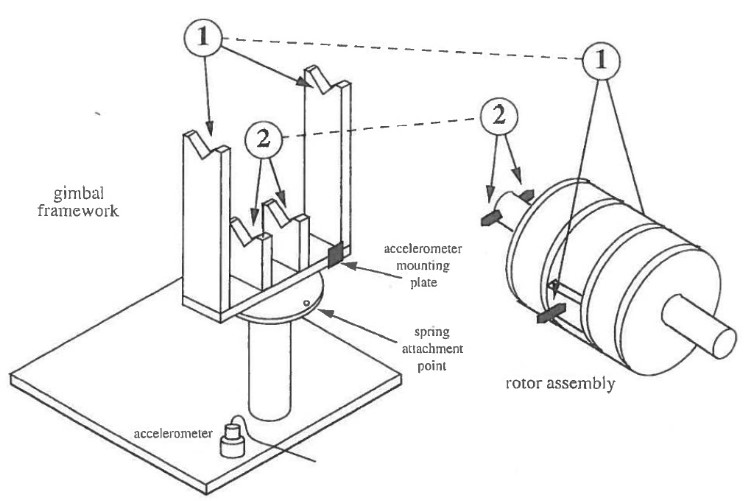
\includegraphics[width=0.5\textwidth]{setup.jpg}
    \caption{Gyroscope assembly}
    \label{fig:setup}
\end{figure}

\section{Theory}

Moment of inertia 

Parallel axis theorem
\begin{equation}
    I_{xx} = I_G + md^2 
\end{equation}

Perpendicular axis theorem
\begin{equation}
    I_{zz} = I_{xx} + I_{yy}
\end{equation}

The dimensions of the rotor can be tabulated as follows:

\begin{table}[H]
    \centering
    \begin{tabular}{|c|c|c|c|}
        \hline
        \multirow{ 2}{*}{Parameter} & \multicolumn{3}{|c|}{Annular Sections} \\
        \cline{2-4}
        & Outer rim & Central Spokes & Inner Rim \\
        \hline
        $r_i$ (mm) & 74 & 26 & 16.5 \\
        $r_o$ (mm) & 85 & 74 & 26 \\
        $L$ (mm) & 63 & 10 & 30 \\
        \hline
        $m$ (kg) & 2.700 & 1.176 & 0.297 \\
        \hline
        $I_{zz}$ (kgm$^2$) & 0.01715	& 0.00362 & 0.00014 \\
        \hline

    \end{tabular}
    \caption{Rotor dimensions}
\end{table}

The mass and moment of inertia of each annulus section is calculated by
\begin{equation}
    m = \frac{\pi}{2} \rho L(r_o^2 - r_i^2), \;\;\;\;\;\; I_{zz} = \frac{\pi}{2} \rho L(r_o^4 - r_i^4)
\end{equation}

These can be added together by parallel axis theorem to give the total moment of inertia of the rotor about the axis of rotation.
Then $C = 2A$ for both the rotor and rotor housing so $I_G = (C + J_1)/2$.
Then the moment of inertia about point 2 as seen in figure \ref{fig:setup} is given by parallel axis theorem as $I_2 = I_G + Mr^2$.

\begin{alignat}{2}
    \text{Mass of rotor} \;\;\;\; & m \approx 4.173 \text{ kg} \nonumber\\
    \text{Total mass of rotor assembly} \;\;\;\; & M \approx 10.8 \text{ kg} \nonumber\\
    \text{Moment of inertia of rotor about its spin axis,} \;\;\;\; &  C \approx 0.02091 \text{ kgm}^2 \nonumber \\
    \text{Moment of inertia of rotor about other axes,} \;\;\;\; &  A \approx 0.01046 \text{ kgm}^2 \nonumber \\
    \text{Moment of inertia of rotor assembly about pin 1,} \;\;\;\; & I_G \approx 0.08400 \text{ kgm}^2 \nonumber \\
    \text{Moment of inertia of rotor assembly about the rotor axis (excluding rotor)} \;\;\;\; &  J_1 \approx 0.0250 \text{ kgm}^2 \nonumber \\
    \text{Moment of inertia of the gimbal frame about its vertical axis of rotation,} \;\;\;\; &  I_1 \approx 0.0160 \text{ kgm}^2 \nonumber \\
    \text{Moment of inertia of the rotor assembly about pin 2,} \;\;\;\; &  I_2 \approx 0.5603 \text{ kgm}^2 \nonumber \\
    \text{Spring constant (nominal) of each of the rate gyro springs} \;\;\;\; & k \approx 500 \text{N/m} \nonumber
\end{alignat}

The radius of gyration of the rotor assembly about pin 1 is given by $r_g = \sqrt{I_G/M}$ and was found to be $88.2$ mm
The radii of gyration of the rotor and rotor frame about pin 1 can be calculated by $r_R = \sqrt{A/m}$ and $r_F = \sqrt{(I_G - A)/(M-m)}$.
Theser were found to be $50.0$ and $105$ mm respectively.
Therefore it makes sense for the assembly to have a radius of gyration between the rotor and rotor frame.
Also because the mass of the frame is much larger than the rotor, the radius of gyration of the assembly is much closer to that of the frame.

\subsection{Dynamics}

% Euler equations
The Euler equations for an AAC gimble with angular velocity $\bm{\omega}$ in its own reference frame.
The angular velocity of the reference frame is given by $\bm{\Omega}$.
\begin{align}
    A\dot{\Omega}_1 - (A\Omega_3 - C \omega_3) \Omega_2 &= Q_1 \tag{A1}\\
    A\dot{\Omega}_2 + (A\Omega_3 - C\omega_3) \Omega_1 &= Q_2 \tag{A2} \\
    C\dot{\omega}_3 &= Q_3 \tag{A3}
\end{align}

In steady precession $Q_1 = Q_3 = 0$, and $\omega_3 >> \Omega_3$.
Using Euler angles in the 
\begin{equation}
    C\omega_3 \Omega_1 = C\omega_3 \dot{\phi} sin \theta = Q \tag{A4} \label{eq:A4}
\end{equation}

For nutation neglecting the effects of gimbal inertia, the first and second gyroscope equations can be linearised to give:
\begin{equation}
    \ddot{\omega_1} + \left[ \frac{C\omega_3}{A} \right]^2 \omega_1 = 0 \;\;\;\;\;\;\;\; \ddot{\omega_2} + \left[ \frac{C\omega_3}{A} \right]^2 \omega_2 = 0 \tag{A5}
\end{equation}
Which both have a frequency of $ f = \frac{C\omega_3}{A} $.

It can be shown that including the effects of gimbal inertia, the nutation frequency is given by
\begin{equation}
    f = \frac{C\omega_3}{I_G} \left( 1 + \frac{J}{I_G}cot^2\theta_0 + \frac{I_1}{I_G}cosec^2\theta_0 \right)^{-\frac{1}{2}} \tag{A7}
\end{equation}
where $I_1$ is the moment of inertia of the gimbal framework (the stand) about its vertical axis
and $J_1$ is the moment of inertia of the rotor assembly about the rotor axis.

\subsection{Rate Gyro}

The Rate Gyro features two springs, A and B attached to the gimbal frame and the rotor assembly.
These springs can apply a torque to the rotor assembly and induce precession.
There exists an equilibrium position where the force in the springs are balanced and so there is no torque on the rotor assembly and thus no precession.

\begin{figure}
    \centering
    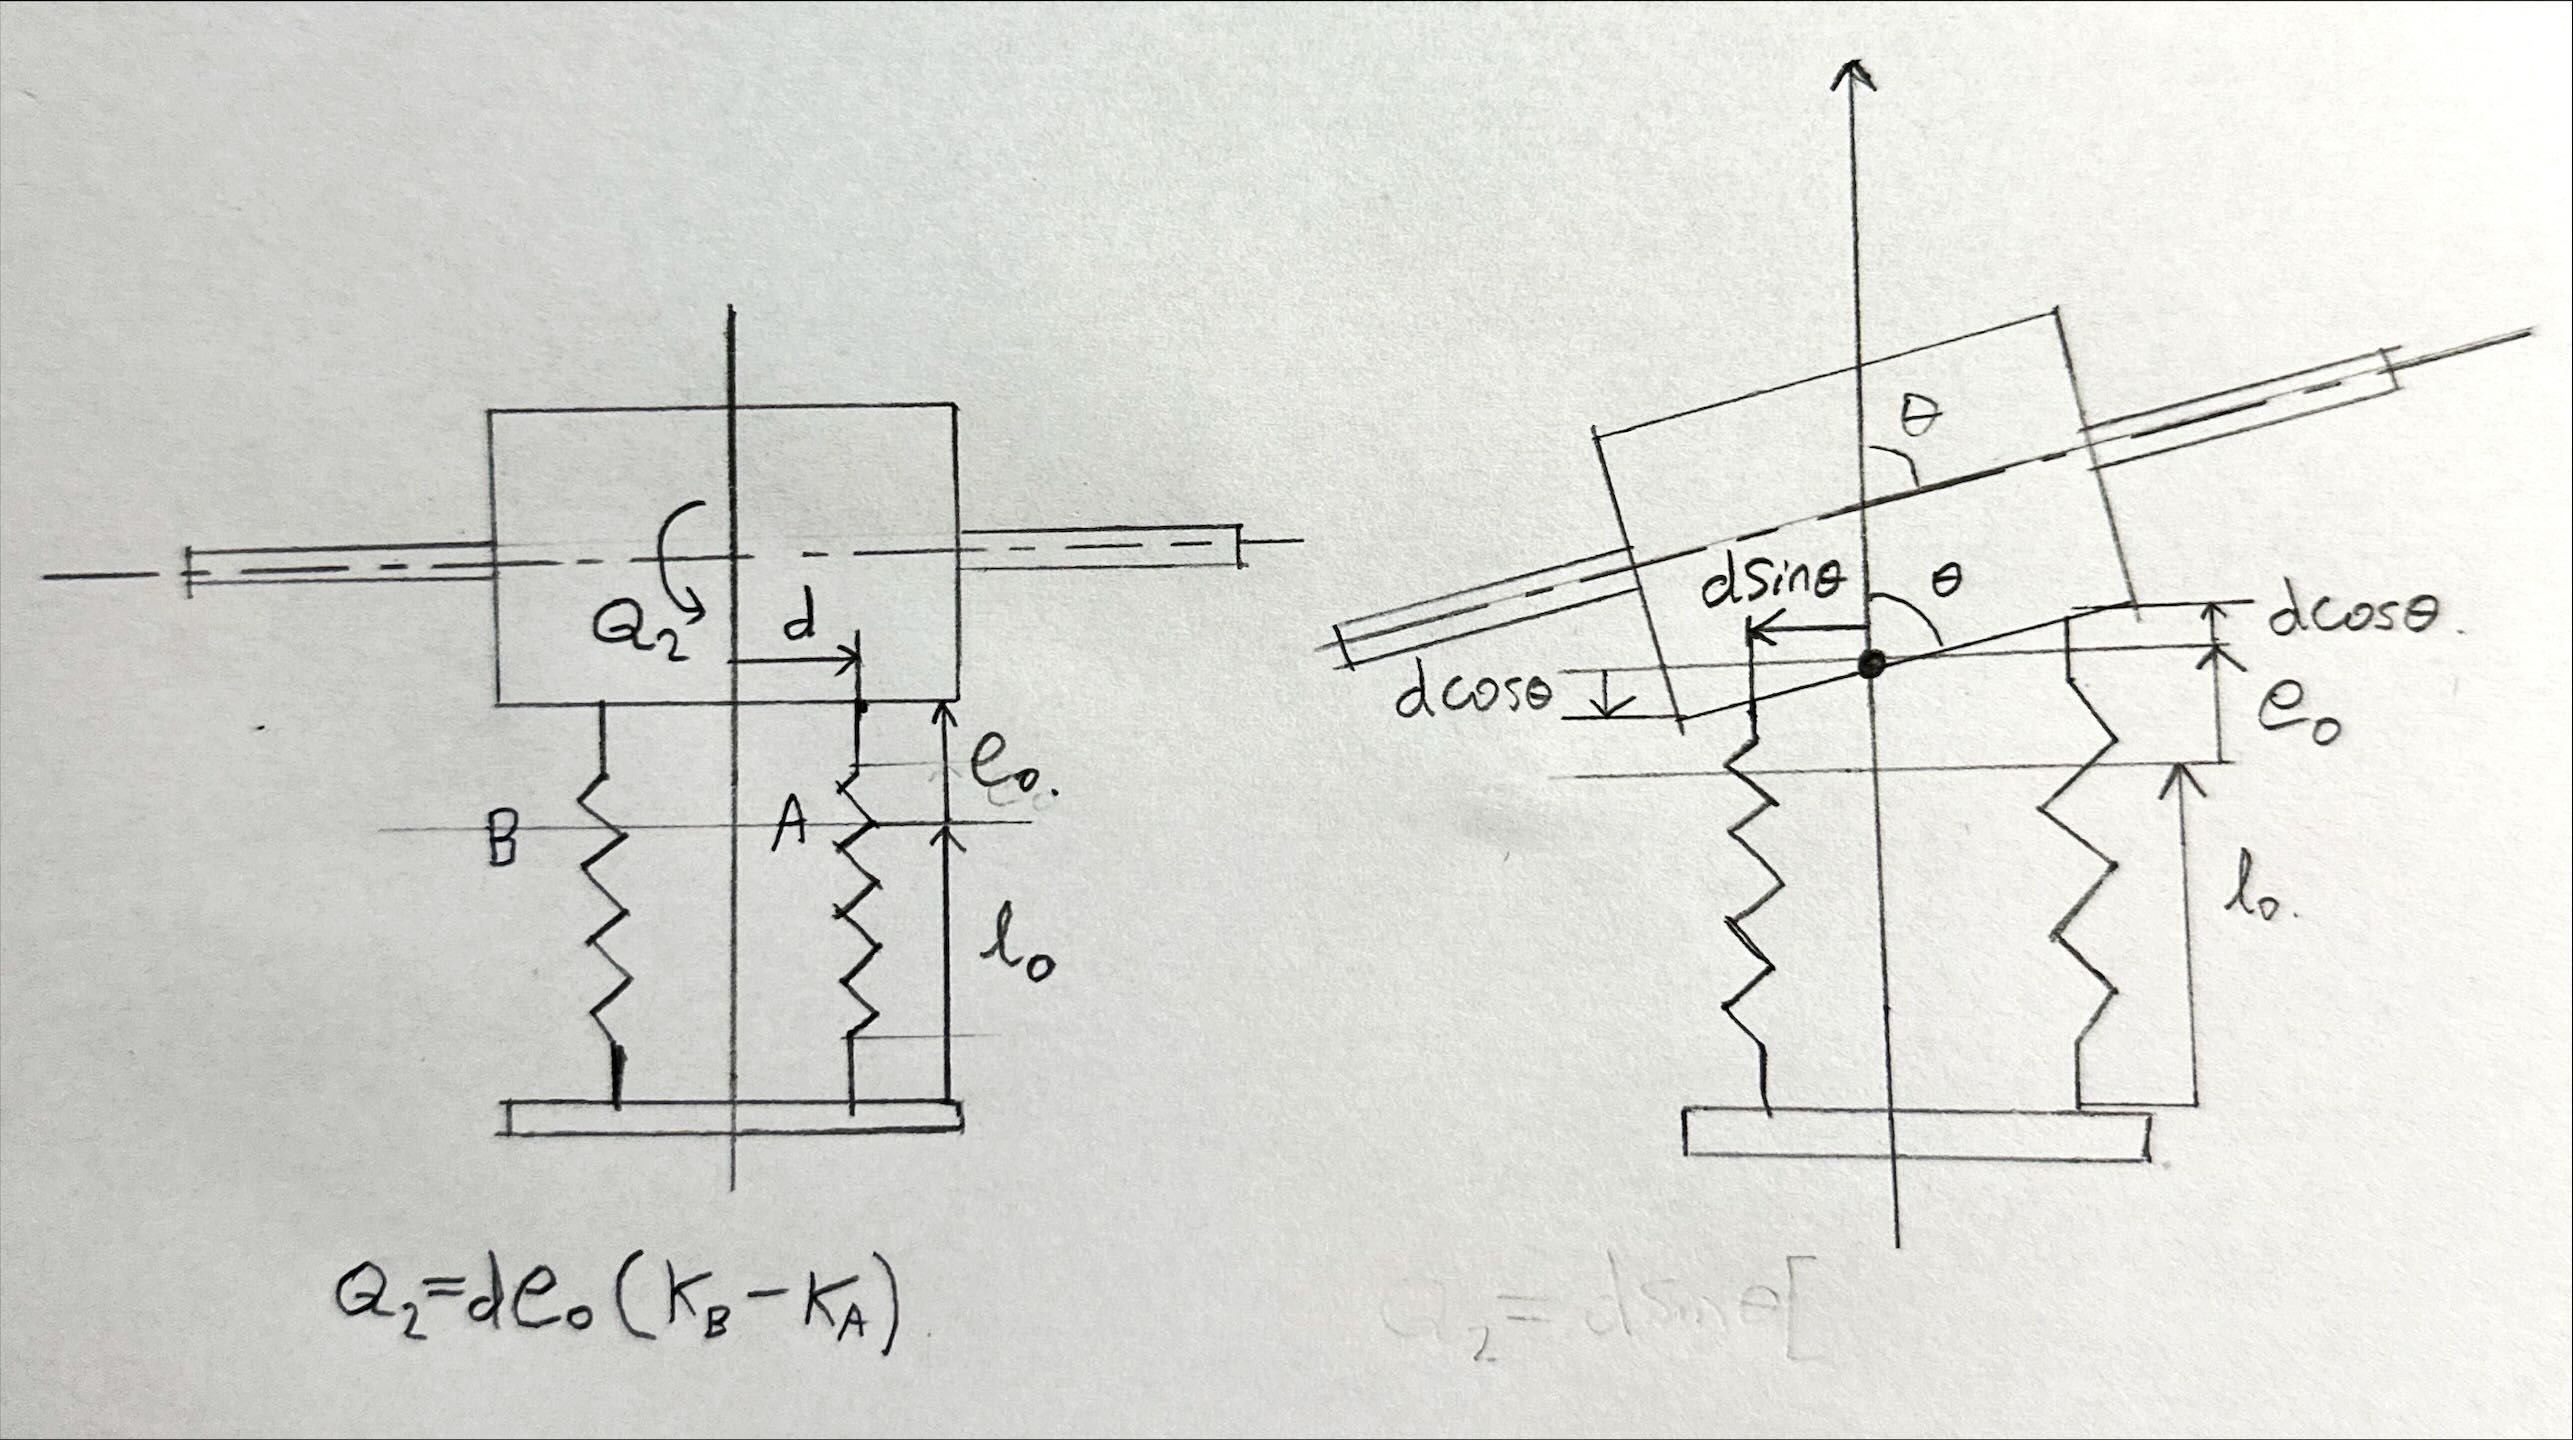
\includegraphics[width=0.5\textwidth]{rate_gyro.jpg}
    \caption{Rate Gyro}
    \label{fig:rate_gyro}
\end{figure}

The spring constants were calculated by simply measuring displacement under a load of $2g$.
The torque due to the springs is given by
\begin{align}
    Q &= d \sin \theta \left[ k_B (e_0 - d \cos \theta) - k_A (e_0 + d \cos \theta) \right] \\
    Q &= d \sin \theta \left[ e_0 (k_B - k_A) - d \cos \theta (k_A + k_B) \right]
\end{align}
Where $d = 0.06$ m is the distance to the center of the rotor assembly and $e_0$ is the extension of the springs at $\theta = 90^o$ which is assumed to be the same for both springs as they have similar unloaded lengths.
However, the springs have varying spring constants $k_A$ and $k_B$, which are determined later.
The value of $e_0$ was not measured !!!?.

\subsection{Cuspidal Nutation}

Cuspidal nutation can be observed when a gyroscopic pendulum is released from rest.

The small angle $\alpha$ through which the rotor tilts during cuspidal nutation is
given by
\begin{equation}
    \alpha \approx \frac{2mgr(I_1+I_2)}{(C\omega_3)^2} \tag{A8}
\end{equation}


\section{Results}

\begin{table}[H]
    \centering
    \begin{tabular}{|c|c|c|c|c|}
        \hline
        Mass (kg) & $Q_{mg}$ (Nm) & Period (s) & $\Omega$ (rad/s) & $Q_{\Omega} $ (Nm) \\
        \hline
        0.5 & 1.03 & 64.72 & 0.09708 & 0.988\\
        1.0 & 2.06 & 33.35 & 0.18840 & 1.918\\
        1.5 & 3.09 & 22.03 & 0.28521 & 2.903\\
        2.0 & 4.12 & 16.78 & 0.37444 & 3.812\\
        \hline
    \end{tabular}
    \caption{Rate of precession with varying mass load at constant $\theta = 90^o$}
    \label{tab:precession_vs_mass}
\end{table}


\begin{table}[H]
    \centering
    \begin{tabular}{|c|c|c|c|c|}
        \hline
        $\theta$ ($^o$) & $Q_{mg}$ (Nm) & Period (s) & $\Omega$ (rad/s) & $Q_{\Omega} $ (Nm) \\
        \hline
        90 & 4.12 & 16.62 & 0.37805 & 3.849\\
        105 & 3.98 & 16.25 & 0.38666 & 3.802\\
        120 & 3.57 & 16.47 & 0.38149 & 3.363\\
        135 & 2.91 & 15.81 & 0.39742 & 2.861\\
        150 & 2.06 & 16.19 & 0.38809 & 1.975\\
        \hline
    \end{tabular}
    \caption{Rate of precession with varying $\theta$ at constant mass load $m = 2.0$ kg}
    \label{tab:precession_vs_theta}
\end{table}

\begin{figure}[H]
    \centering
    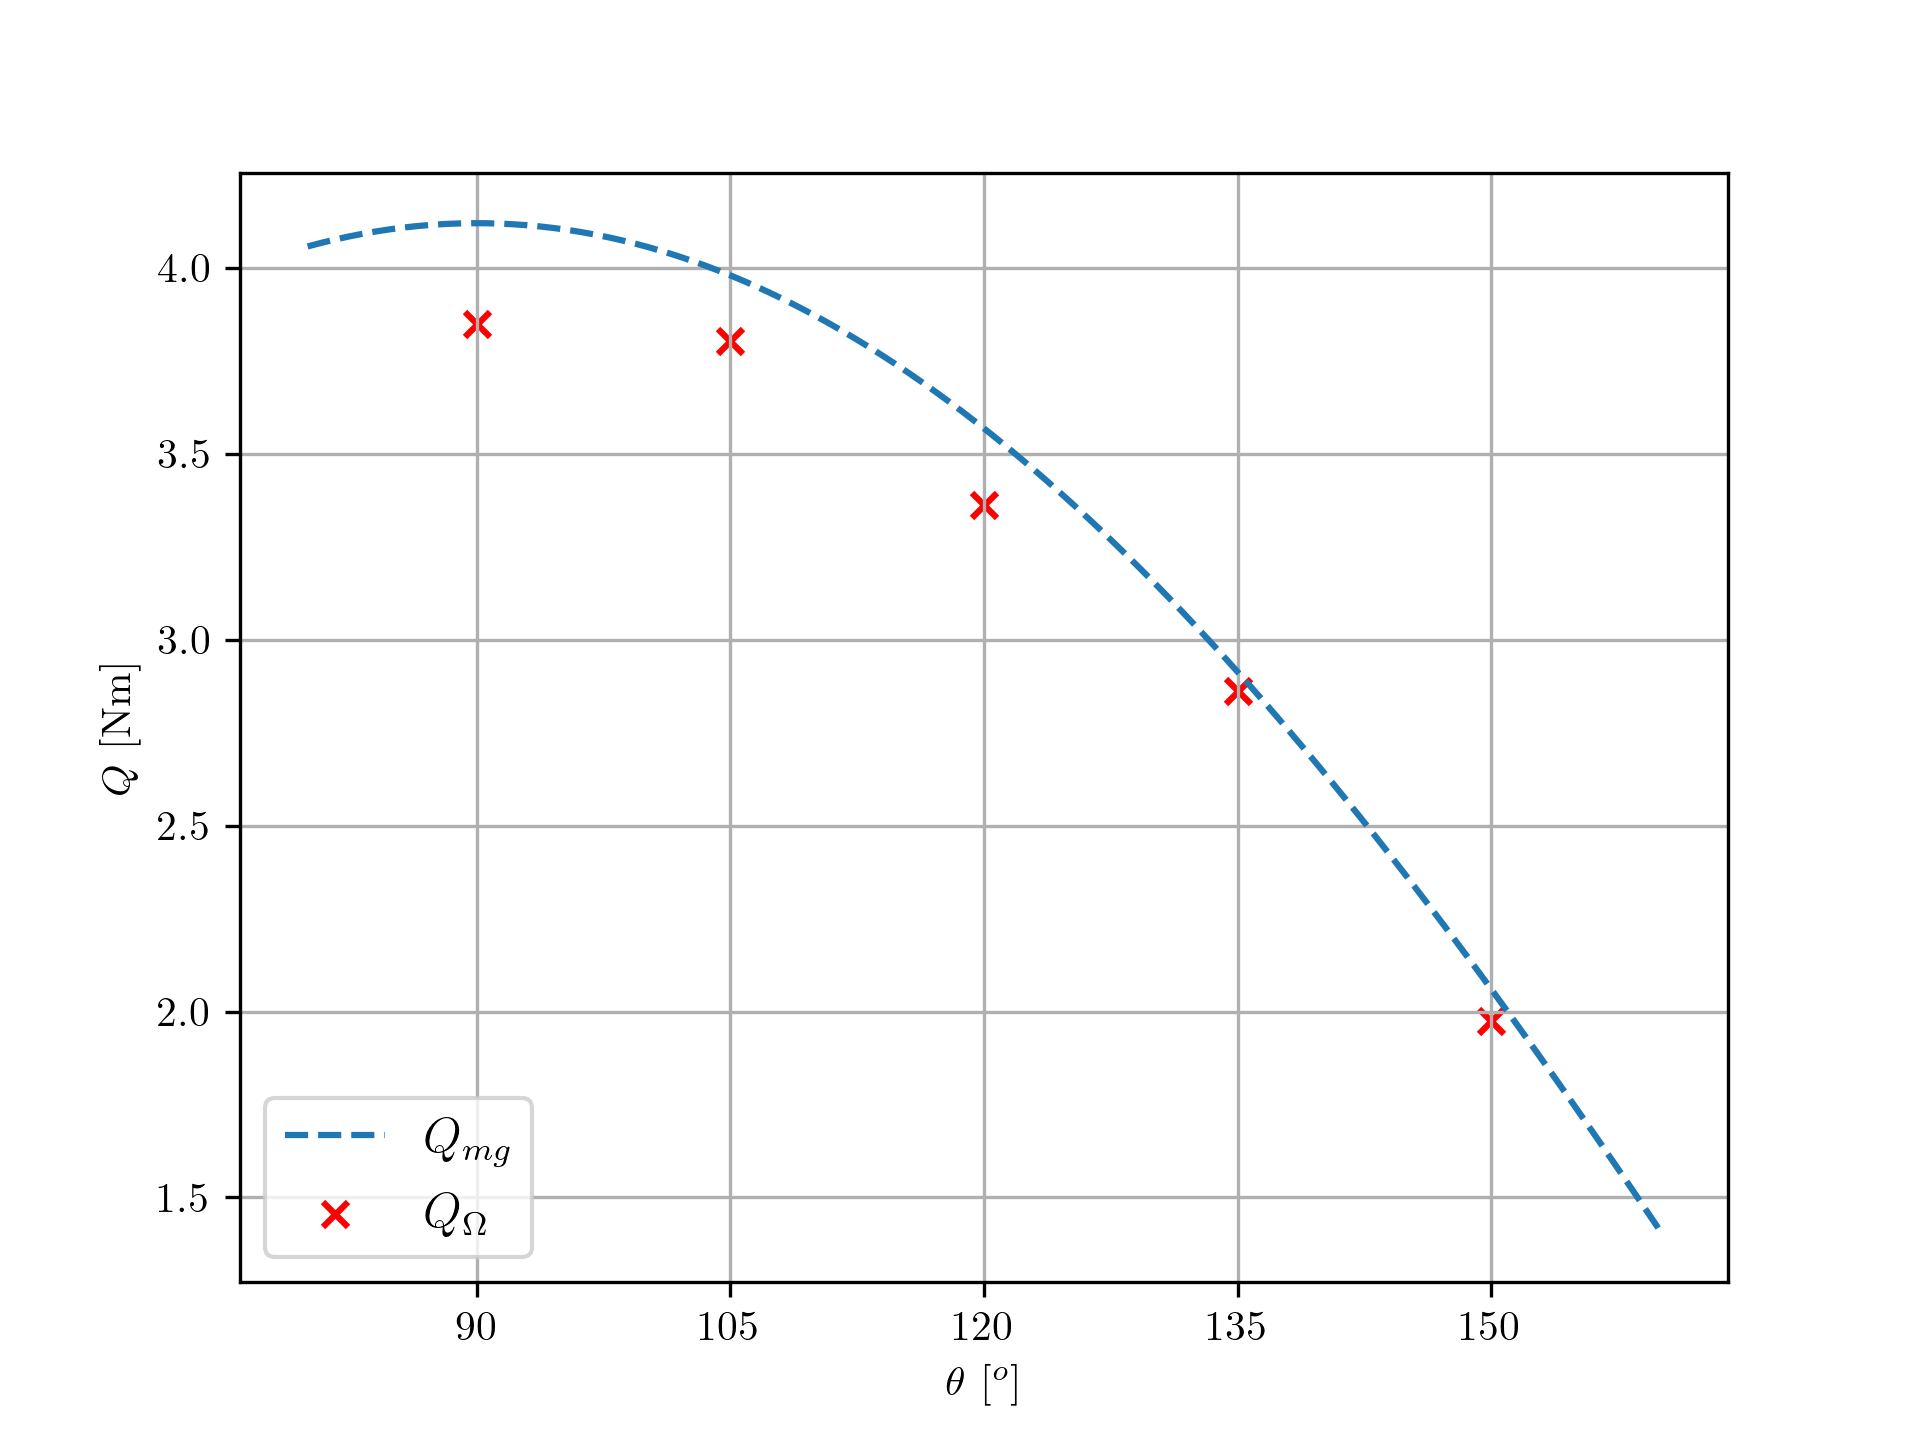
\includegraphics[width=0.5\textwidth]{precession_vs_theta.png}
    \caption{Torque calculated from precession rate for varying $\theta$ for a constant mass load $m = 2.0$ kg}
    \label{fig:precession_vs_theta}
\end{figure}

% nutation frequencies
% trial angle meas_freq calc_freq_without_gimbal calc_freq_with_gimbal

\begin{table}[H]
    \centering
    \begin{tabular}{|c|c|c|c|}
        \hline
        Trial & $\theta$ ($^o$) & $f_{\text{meas}}$ (Hz) & $f_{(A7)}$ (Hz) \\
        \hline
        1	& 90   &	17.2    & 	17.678 \\
        2	& 105  &	17.8    & 	17.423 \\
        3	& 105  &	15.6    & 	17.423 \\
        4	& 120  &	16.1    & 	16.581 \\
        5	& 120  &	15.1    & 	16.581 \\
        6	& 120  &	1.53    & 	16.581 \\
        7	& 120  &	14.7    & 	16.581 \\
        8	& 135  &	15.6    & 	14.887 \\
        9	& 135  &	8.47    & 	14.887 \\
        10	& 135  &	8.2	    &   14.887 \\
        11	& 135  &	7.69    & 	14.887 \\
        12	& 150  &	6.94    & 	11.838 \\
        13	& 150  &	1.54    & 	11.838 \\
        14	& 150  &	1.6	    &   11.838 \\
        15	& 150  &	14.7    & 	11.838 \\
        \hline
    \end{tabular}
    \caption{Calculated and measured nutation frequency for varying $\theta$.}
    \label{tab:nutation}
\end{table}

\begin{figure}[H]
    \centering
    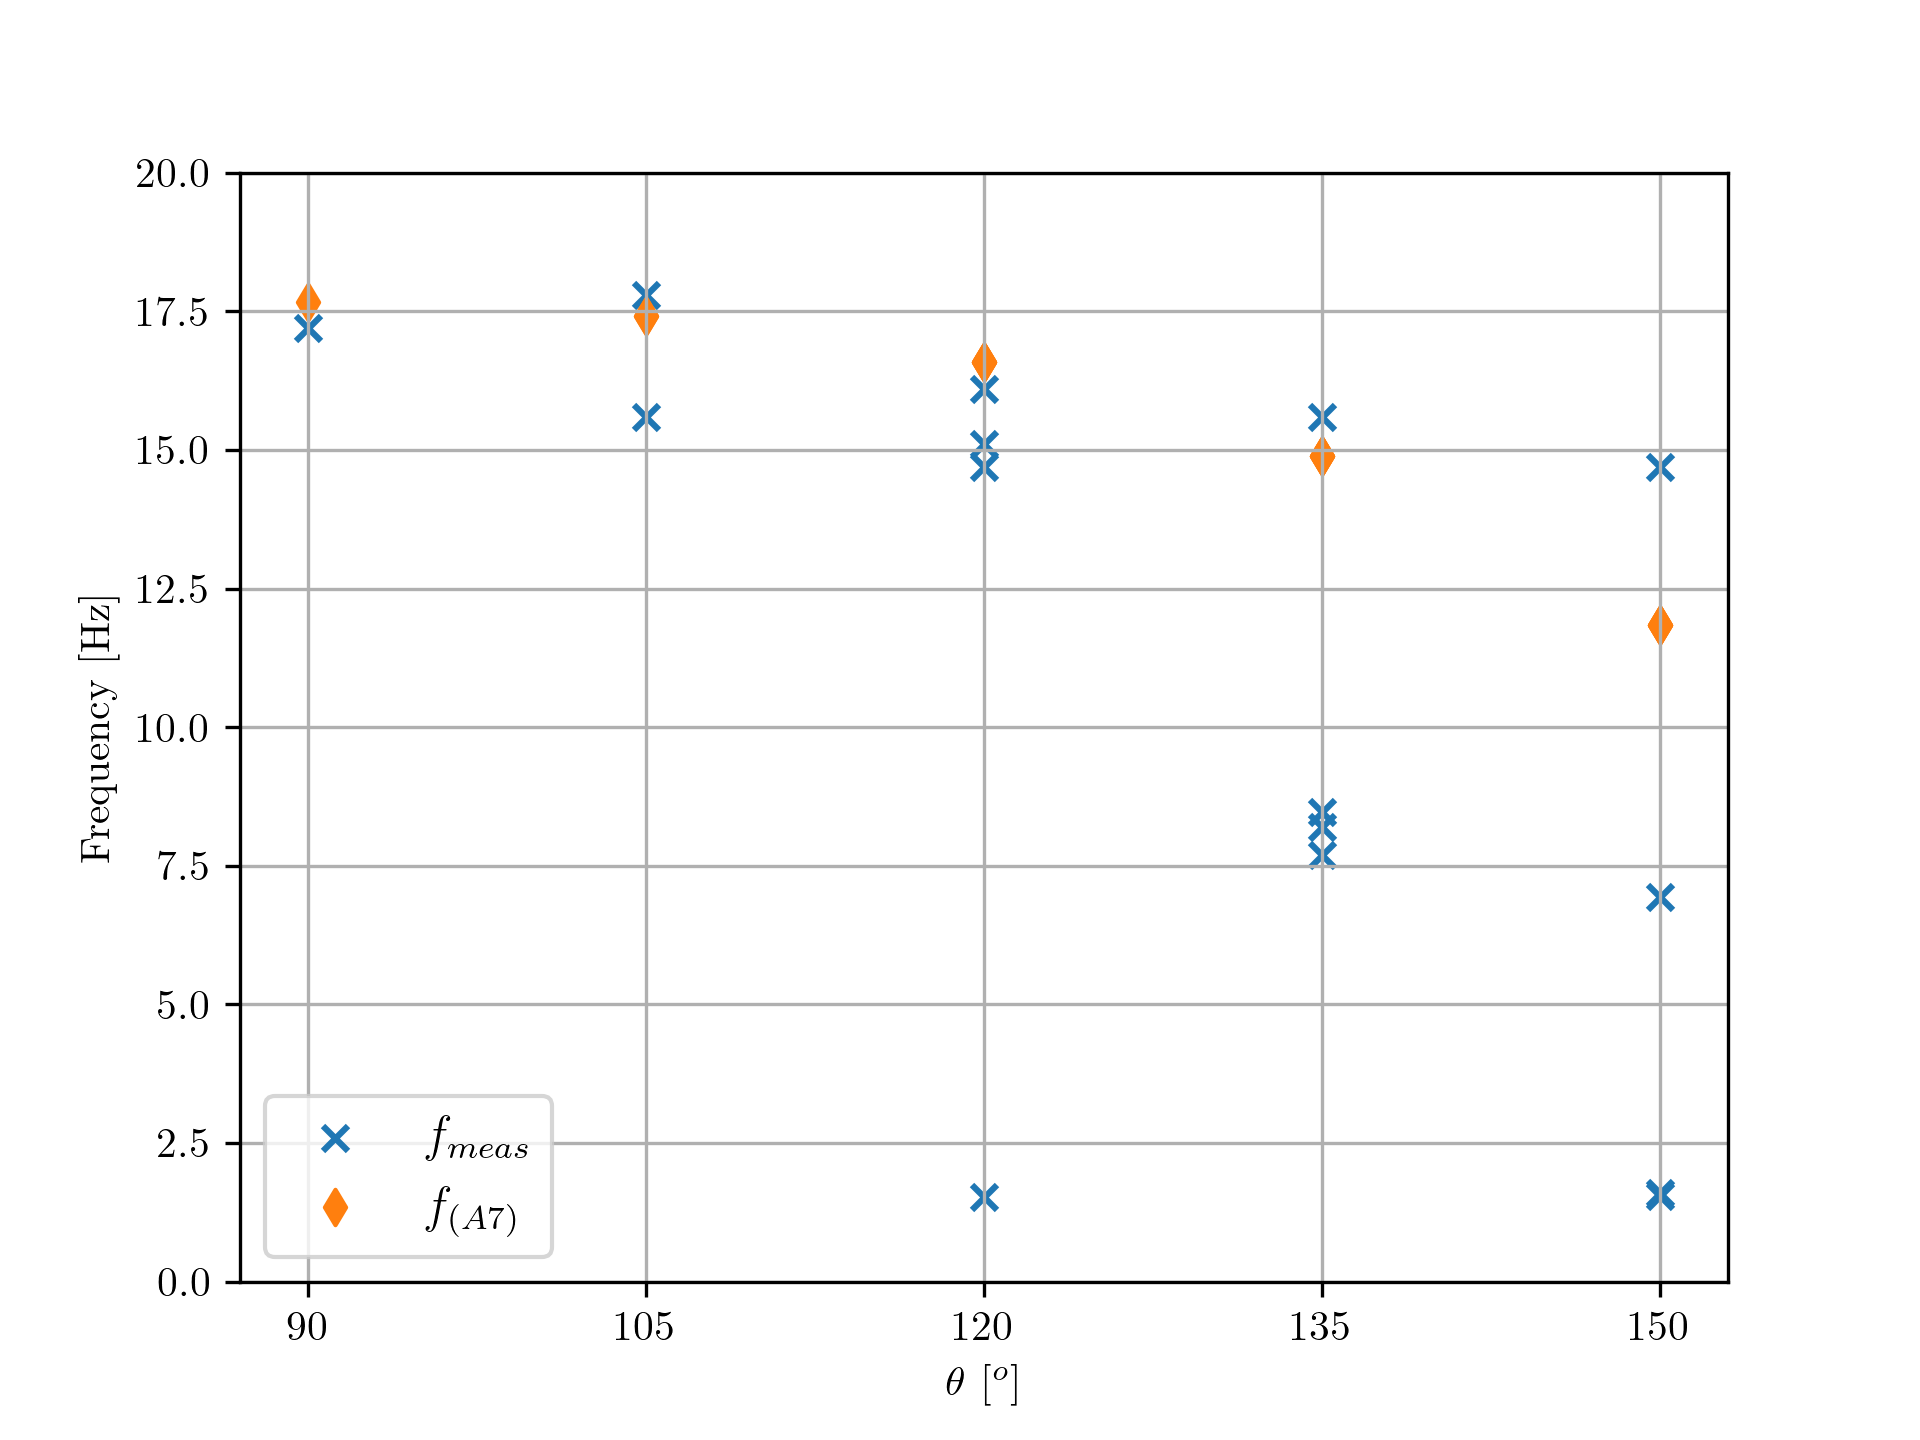
\includegraphics[width=0.5\textwidth]{nutation.png}
    \caption{Nutation frequency with varying $\theta$}
    \label{fig:nutation}
\end{figure}

% rate Gyro and spring constants

\begin{table}[H]
    \centering
    \begin{tabular}{|c|c|c|c|c|}
        \hline
        Spring & $l_0$ (m) & $l$ (m) & $F$ (N) & $k$(N/m)\\
        \hline
        A	& 0.133	& 0.158	& 19.62	& 785 \\
        B	& 0.132	& 0.162	& 19.62	& 654 \\
        \hline
    \end{tabular}
    \caption{Rate of precession with varying spring constant $k$}
    \label{tab:springs}
\end{table}

\begin{table}[H]
    \centering
    \begin{tabular}{|c|c|c|c|c|}
        \hline
        $\theta$ ($^o$) & Period (s) & $\Omega_3$ (rad/s) &  $Q_{(A4)}$ (Nm)\\
        \hline
        105	& 20.91	& 0.3004871022  &	2.955 \\
        75	& 19.13	& -0.3284466967	&   -3.230 \\
        \hline
    \end{tabular}
    \caption{Rate Gyro}
    \label{tab:precession_vs_k}
\end{table}

% Cuspidal nutation,
% trial angle period nutations frequency

\begin{table}[H]
    \centering
    \begin{tabular}{|c|c|c|c|c|}
        \hline
        Trial & $\theta$ ($^o$) & Nutations  & Period (s) & Frequency (Hz)\\
        \hline
        1   & 30	& 6	    &   3.16	& 1.899 \\
        2   & 30    & 6	    &   2.9	    & 2.069 \\
        3   & 30    & 7	    &   2.83	& 2.473 \\
        4   & 60	& 8	    &   2.84	& 2.817 \\
        5   & 60    & 7	    &   3.16	& 2.215 \\
        6   & 60    & 8	    &   2.96	& 2.703 \\
        7   & 90	& 10    &   4.00	& 2.500 \\
        8   & 90    & 8	    &   2.96	& 2.703 \\
        9   & 90    & 8	    &   3.09	& 2.589 \\
        \hline
    \end{tabular}
    \caption{Measured cuspidal nutation frequency for varying $\theta$.}
    \label{tab:cuspidal_nutation}
\end{table}

\begin{figure}
    \centering
    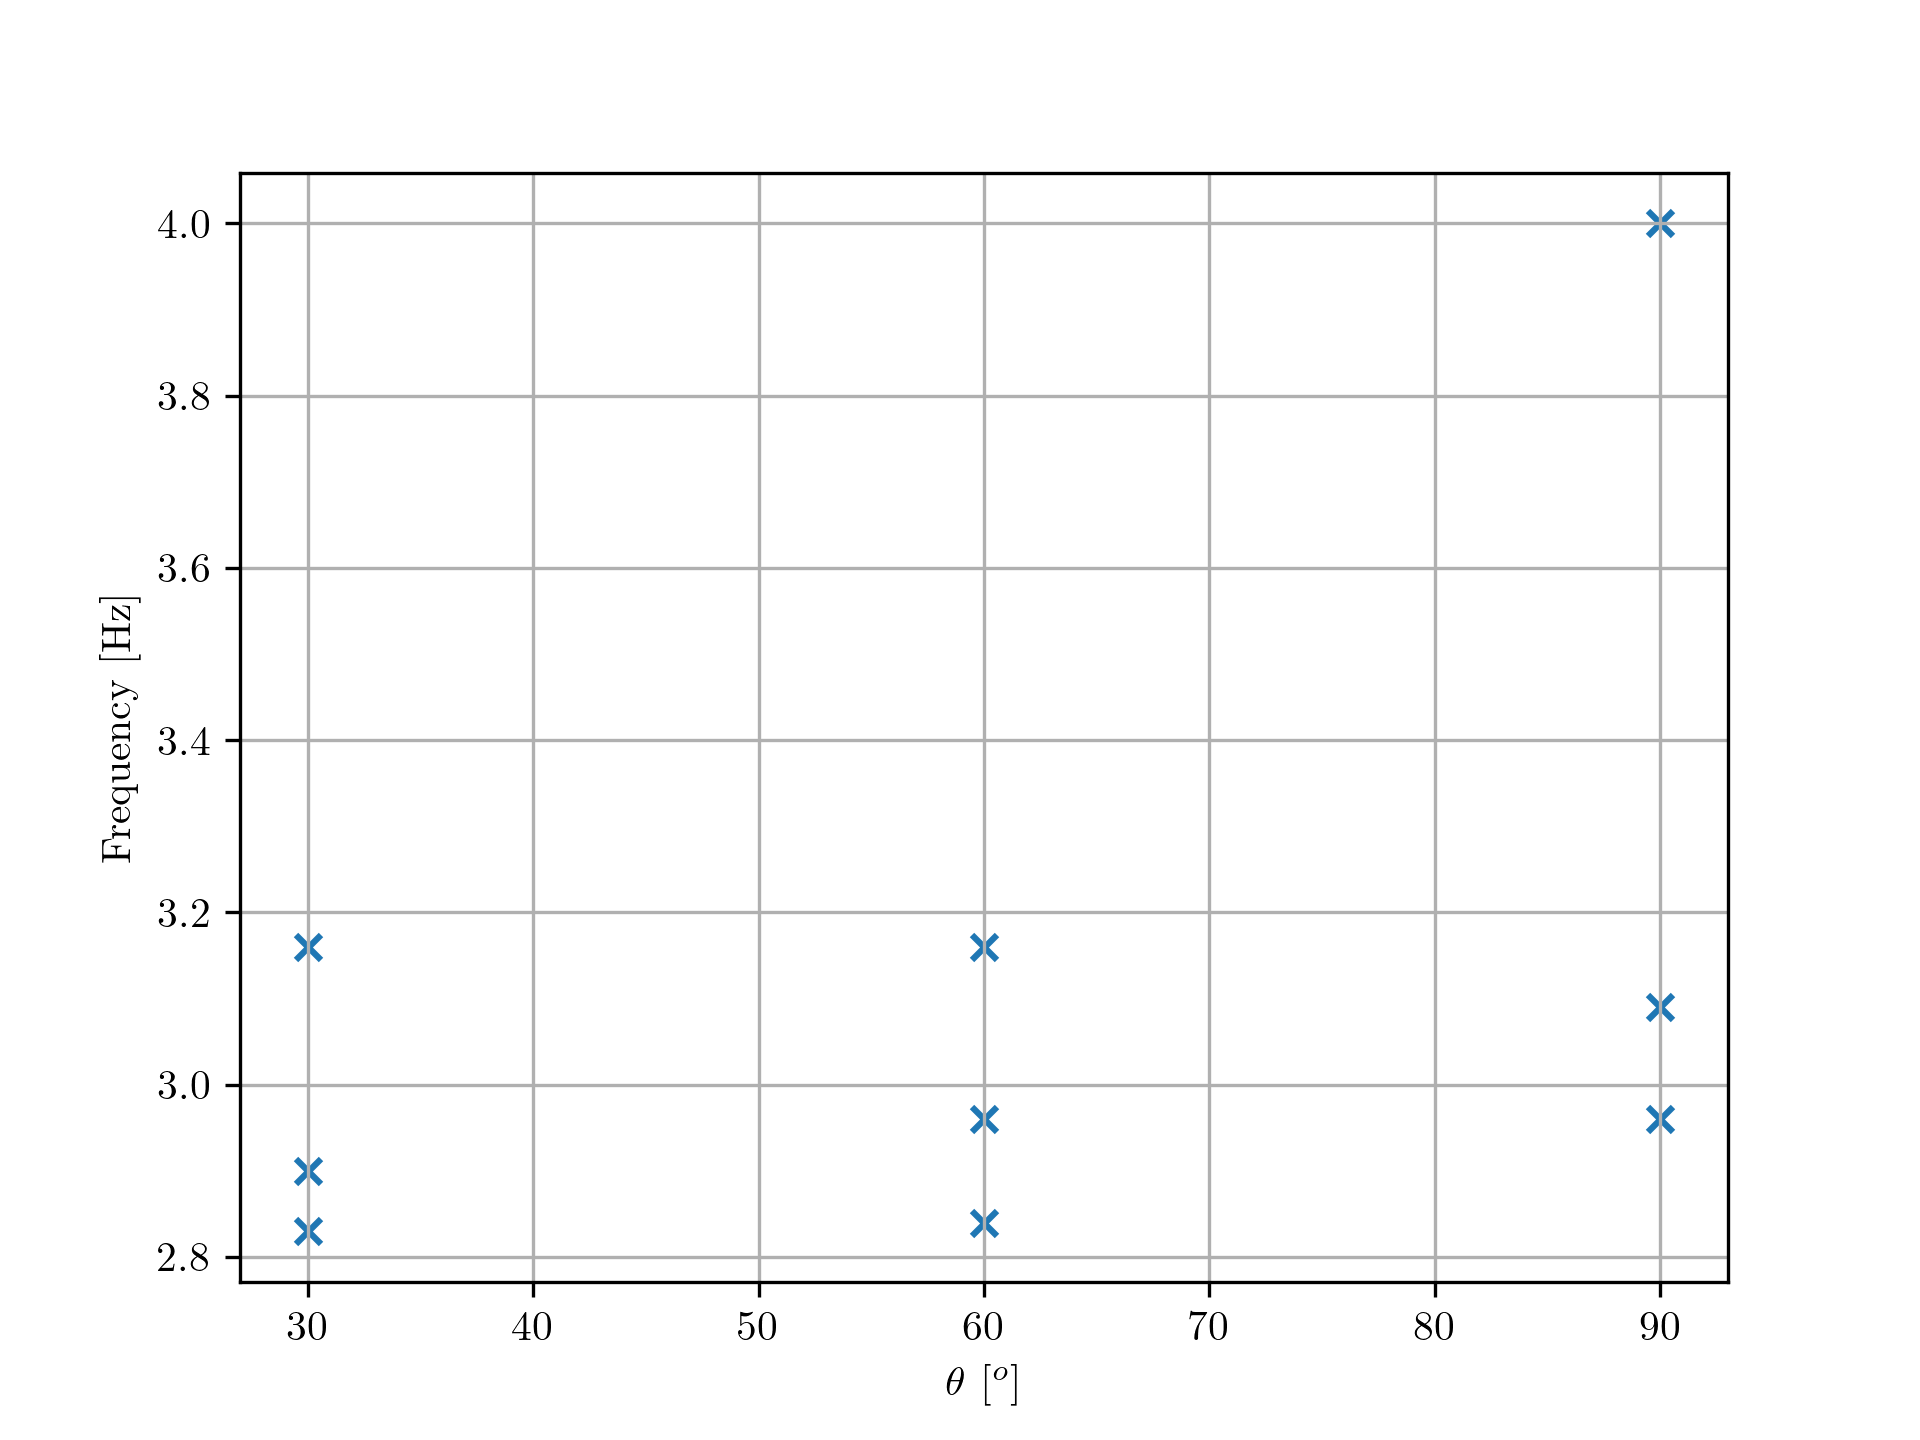
\includegraphics[width=0.5\textwidth]{cuspidal_nutation.png}
    \caption{Cuspidal nutation frequency with varying $\theta$}
    \label{fig:cuspidal_nutation}
\end{figure}

\section{Discussion}

\begin{figure}[H]
    \centering
    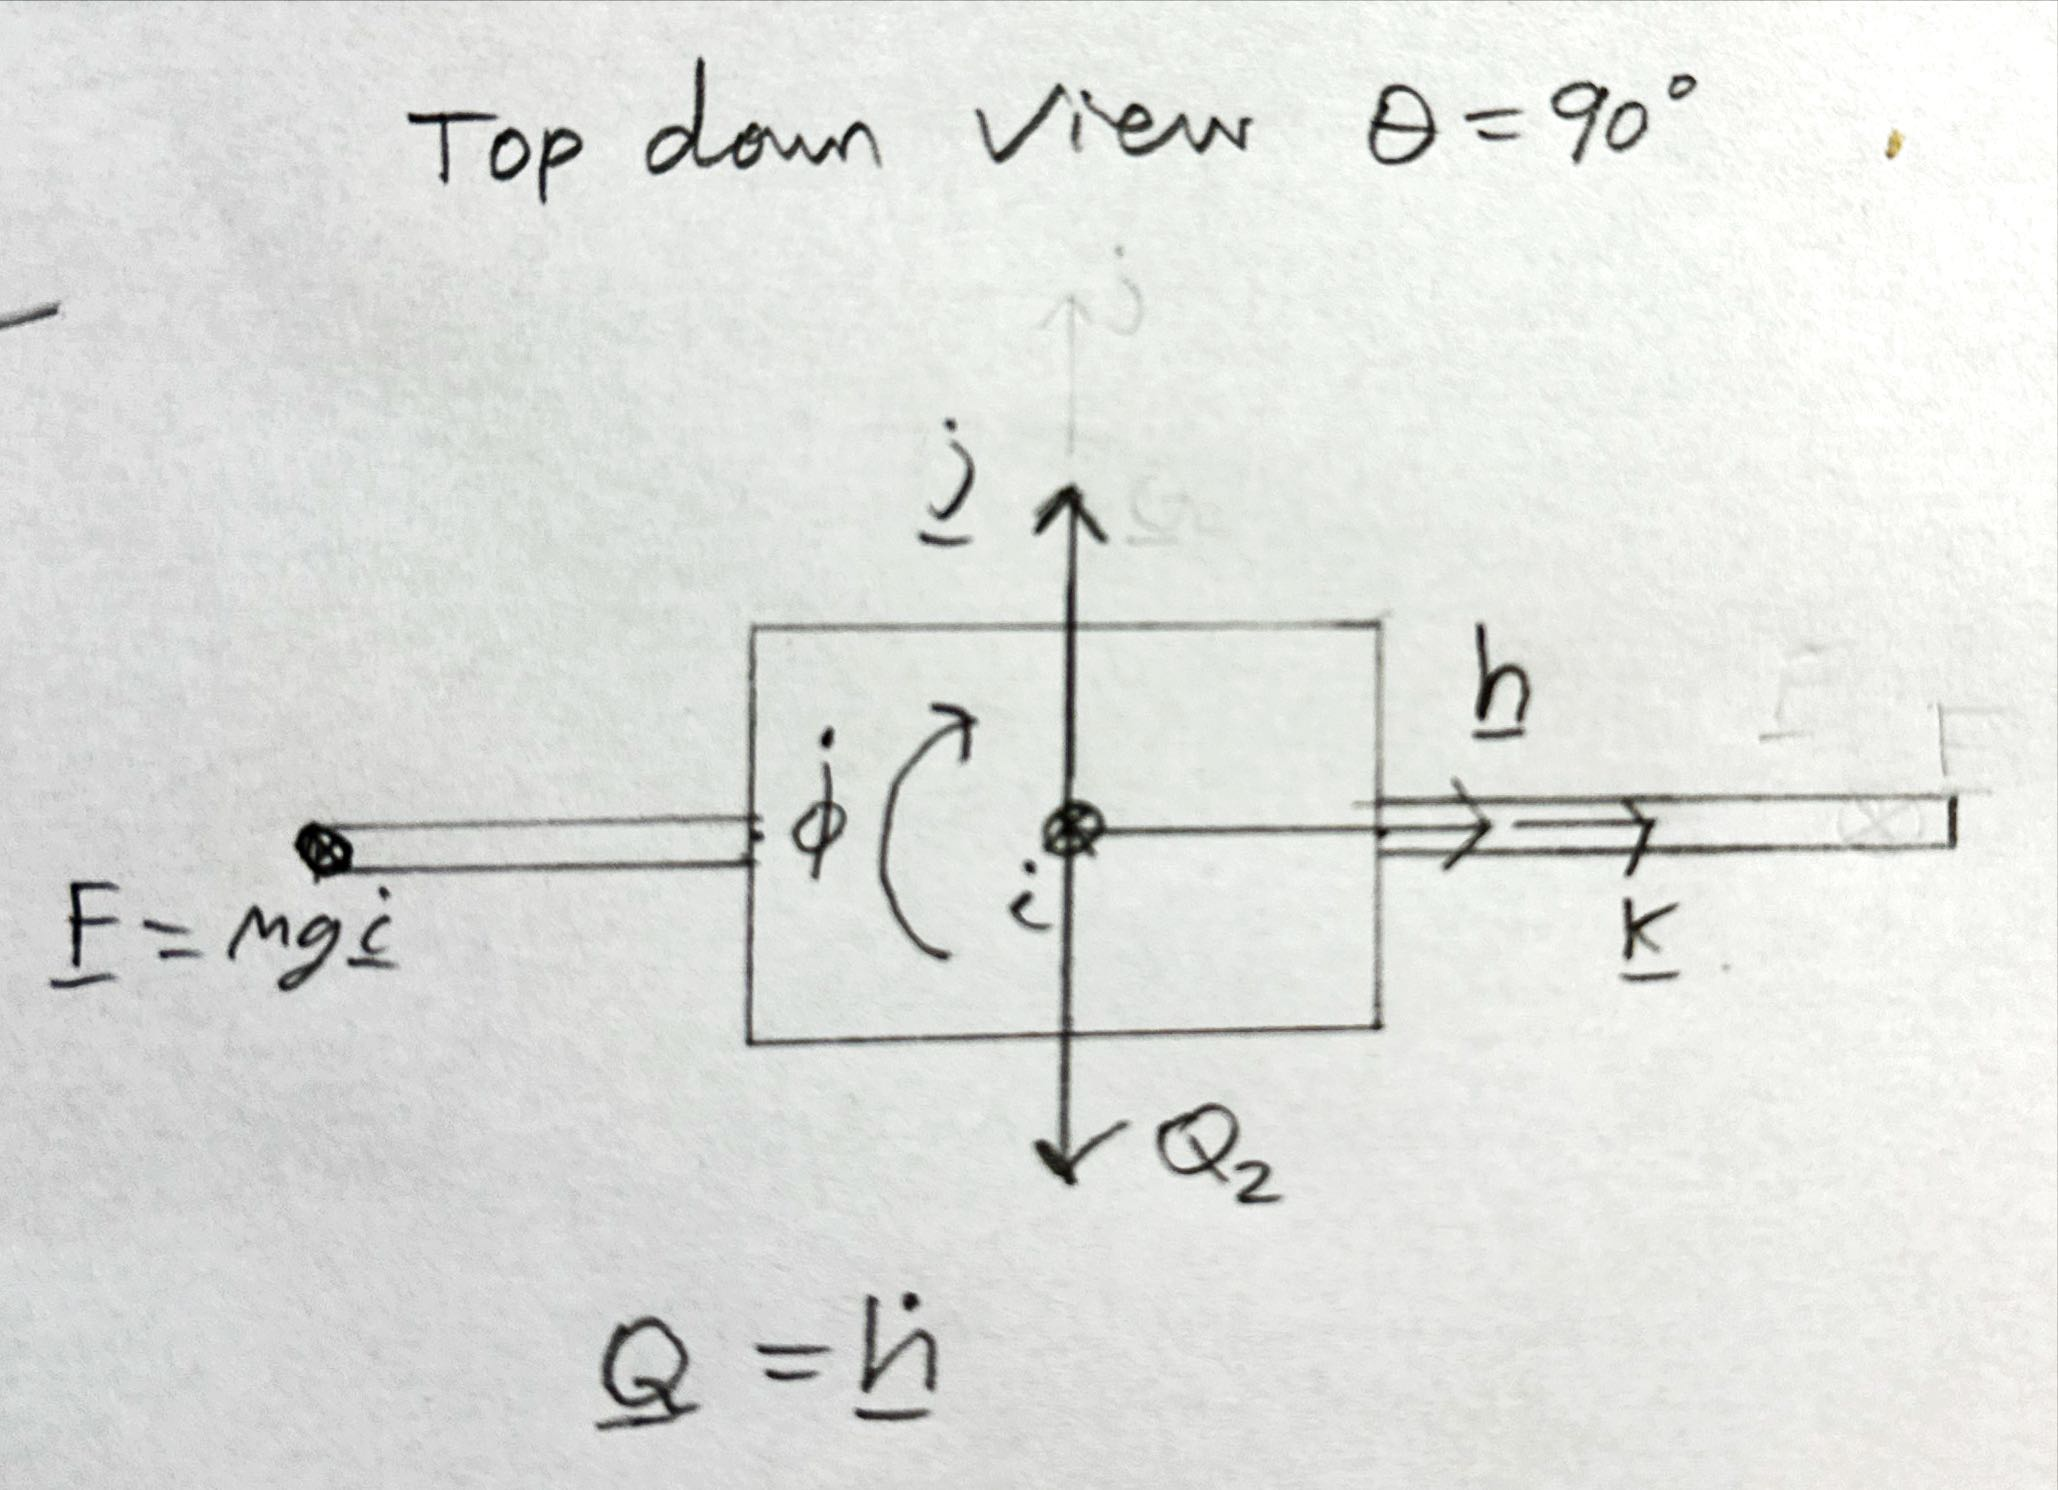
\includegraphics[width=0.5\textwidth]{top_down_precession.jpg}
    \caption{Top down view of steady precession with $\theta = 90^o$}
    \label{fig:precession_vs_mass}
\end{figure}

%%% Steady Precession

% Q1: In what direction should gyroscopic precession occur? 
% Hint: sketch a vector diagram based on Q = ˙h
The direction of precession depends both on the direction of applied torque and the direction of the angular momentum of the rotor.
The torque is equal the rate of change of angular momentum, which causes the angular momentum vector to precess.


% Q2 What is holding the 1kg mass up? Draw a free-body diagram
The 1kg mass applies a torque that is always perpendicular to the angular momentum of the rotor.
This torque is the rate of change of angular momentum of the rotor, and so the angular momentum vector rotates in the direction of the torque but does not change in magnitude.
This can be thought as being similar to circular motion, where a centripetal force is responsible for the change in direction but not the magnitude of the velocity.
The vertical forces are simply balanced by reactions from the gimbal frame and rotor housing.

% Q3: Using equation (A4) calculate what the precession rate 
% should be and time it with a stopwatch.
Table \ref{tab:precession_vs_mass} shows the rate of precession with varying mass load at constant $\theta = 90^o$.
It can be seen that the calculated torques from measured precession rate (\ref{eq:A4}) are within 8\% of the torques applied by the masses.
This discrepancy was observed to increase with precession rate, as the uncertainty in the period measurement becomes more significant.
There is also some uncertainty in the rotor spin rate, tilt angle of the gyro and the moment of inertia of the rotor.


% Q4: According to the equation how should the rate of precession change when to alter the
% angle of tilt of the gyro? Confirm this result by measuring the precession rate at various tilt
% angles
Figure Table \ref{tab:precession_vs_theta} shows the rate of precession with varying $\theta$ at constant mass load $m = 2.0$ kg.
The line for calculated torque from mass load with angle shows a $sin(\theta)$ relationship.
The precession rate was found to be constant within the error of the period measurement.
This was expected as the sin terms in equation \ref{eq:A4} cancels with the gravity term.
There is larger error at higher values of torque as seen in figure \ref{fig:precession_vs_theta}.
This is again likely due to the uncertainty in the period measurement and the rotor spin rate.
Performing the experiment again with a smaller mass would increase the period of rotation and reduce the uncertainty in the period measurement.

%%% Nutation

% Q6: Use equations (A6) and (A7) with A = IG to calculate the nutation frequency, and
% use the oscilloscope to measure the frequency (there is an accelerometer which you can use to
% measure the nutation vibration, see Fig. 2)
% Q7: Does the nutation rate depend on inclination? Use (A7) to check this out. Tabulate your
% findings

Figure \ref{fig:nutation} shows the calculated and measured nutation frequency for varying $\theta$.
It can be seen that the measured nutation frequencies vary significantly for measurements at the same angle.
??? Im not sure why this is.

%%%% The Rate Gyro

% Q8: Set the gimbal framework rotating about
% the vertical axis at a slow steady speed. What
% do you observe? Use equation (A4) to determine 
% the couple Q2 which must be acting on
% the rotor. What do you estimate is the force in
% each of the springs? Does this make sense?

Table \ref{tab:springs} shows the spring constants for both springs of the rate gyro.
The extension at $\theta = 90^o$ was measured to be 4 cm and so the force in each spring is calculated and shown in the table.

% Q9: How might this device be useful for navigation? 
% Imagine you are at sea on a very foggy day.
The rate gyro can be used to measure the rate of turn of a vehicle as the angle $\theta$ is proportional to the rate of turn.


%%% The gyroscopic pendulum

% Q10 What is holding the gyro up? Draw a free-body diagram. And what is the direction of
% precession? Is it the same as you observed in Q1 ?

For the gyroscopic pendulum case there is a torque acting due to the weight of the rotor and frame.



% Q11 Use a stopwatch to measure the precession rate at various angles. Compare your measurements
% with calculation - plot graphs or tabulate your findings. the battery will be
% getting tired by now - keep an eye on the RPM

% need data for this

% Q12: Take a look at the nutation frequency at different angles. Note that the frequency is low
% enough now to time it with a stopwatch. How do your measurements tie up with calculation
% from formula (A7)



% Q13: When released from horizontal, you get ”cuspidal nutation”. Estimate the angle that
% the gyro drops from the horizontal and see if it tallies with equation (A8). And when the
% oscillations have died out you will notice that the gyro is still tilted a bit downwards. Why?
% Can you work out this angle by using conservation of angular momentum? Sketch a graph of
% the tilt angle - don’t just copy Fig. 8 because there is dissipation in the real world.

\section{Conclusion}



\end{document}
